% Figure from MATH 556 notes, section 5. Compile with the notes preamble.
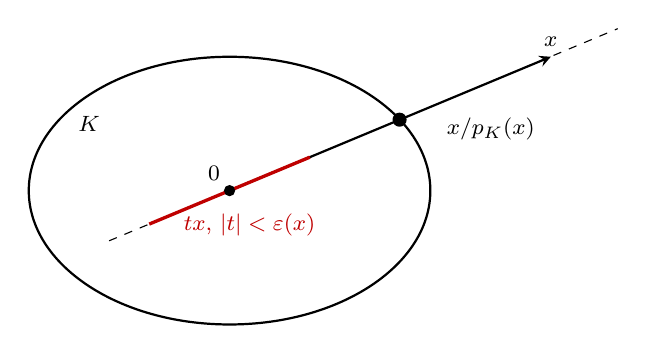
\begin{tikzpicture}[scale=1.7, >=stealth]
    \draw[thick] (0,0) ellipse (1.5 and 1.0);
    \node[font=\footnotesize] at (-1.05,0.5) {$K$};
    \draw[dashed] (-0.9,-0.375) -- (2.9,1.21);
    \draw[->, thick] (0,0) -- (2.4,1.0) node[above, font=\footnotesize] {$x$};
    \draw[very thick, red!75!black] (-0.6,-0.25) -- (0.6,0.25);
    \node[below, font=\footnotesize, red!75!black] at (0.15,-0.1) {$tx$, $|t|<\varepsilon(x)$};
    \fill (1.27,0.53) circle (1.5pt);
    \node[anchor=west, font=\footnotesize] at (1.55,0.46) {$x / p_K(x)$};
    \fill (0,0) circle (1.2pt) node[above left, font=\footnotesize] {$0$};
\end{tikzpicture}
